\pdfminorversion=4
%\documentclass[handout,13pt,aspectratio=169]{beamer}
\documentclass[13pt,aspectratio=43]{beamer}
\usepackage[utf8]{inputenc}

\usetheme{metropolis}

\usepackage{appendixnumberbeamer}
% \usepackage[italian]{babel}
% \usepackage[english]{babel}
\title{
	Performance analysis for TCP BBR in Mininet
}

\date{\today}
\author{Massimo Girondi}
%\titlegraphic{\center\includegraphics[height=2cm]{unitn_trasp.pdf}\\
%\footnotesize Dipartimento di Informatica e Scienza dell'Informazione}
%\metroset{background=dark}


\begin{document}

\maketitle
%\begin{frame}{Table of contents}
%  \setbeamertemplate{section in toc}[sections numbered]
%  \tableofcontents[hideallsubsections]
%\end{frame}

\begin{frame}{TCP BBR (from English Wikipedia)}
	\begin{itemize}
		\item \textbf{B}ottleneck \textbf{B}andwidth and \textbf{R}ound-trip propagation time
		\item Developed by Google in 2016
		\item OpenSource
		\item For YouTube, BBR yielded an average of 4\% higher network throughput (up to 14\%)
		\item Available in Linux Kernel from version 4.9
		\item Seems not too fair to non-BBR streams (cit. Geoff Huston)
	\end{itemize}
\end{frame}

\begin{frame}{Test environment}
	\begin{itemize}
		\item Mininet 2.3 on Debian 9
		\item Virtual machine running on VirtualBox
		\item Provisioned through Vagrant 
		\item Switched star network, Gigabit links with 5ms delay
        \item 4 machines, only two used for tests
		\item Congestion protocol changes for every machine: kernel is shared
	\end{itemize}
\end{frame}
\begin{frame}{Topology}
  \begin{figure}
	  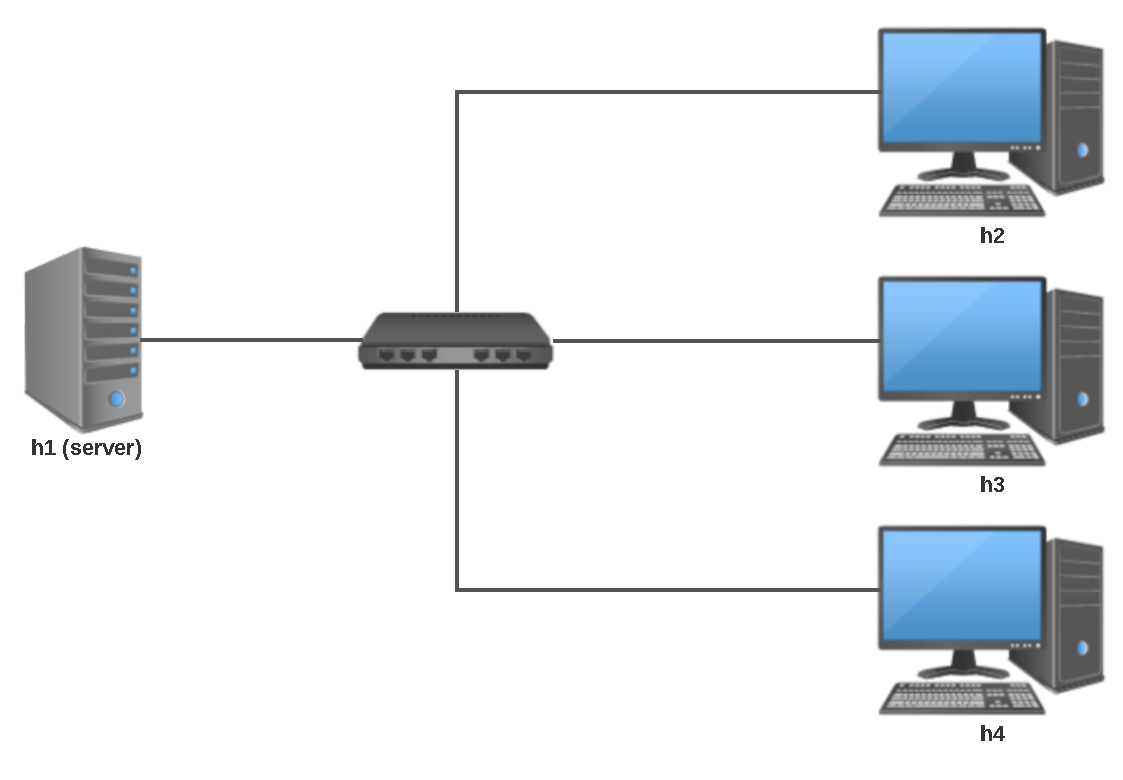
\includegraphics[width=\textwidth,height=\textheight,keepaspectratio]{network.pdf}
  \end{figure}
\end{frame}

\begin{frame}{20 seconds Iperf test: description [1/3]}
	\begin{itemize}
		\item Variable loss rate on the server's link, then variable delay
		\item \texttt{h1} as server
		\item \texttt{h2} as client
		\item Client options: \texttt{-f k -c IP -t 20 }
			\begin{itemize}
				\item[-f k] kbps as output format
				\item[-t 20] Run for 20 seconds
			\end{itemize}
	\end{itemize}
\end{frame}

\begin{frame}{20 seconds Iperf test: speed vs loss (log) [2/5]}
  \begin{figure}
	  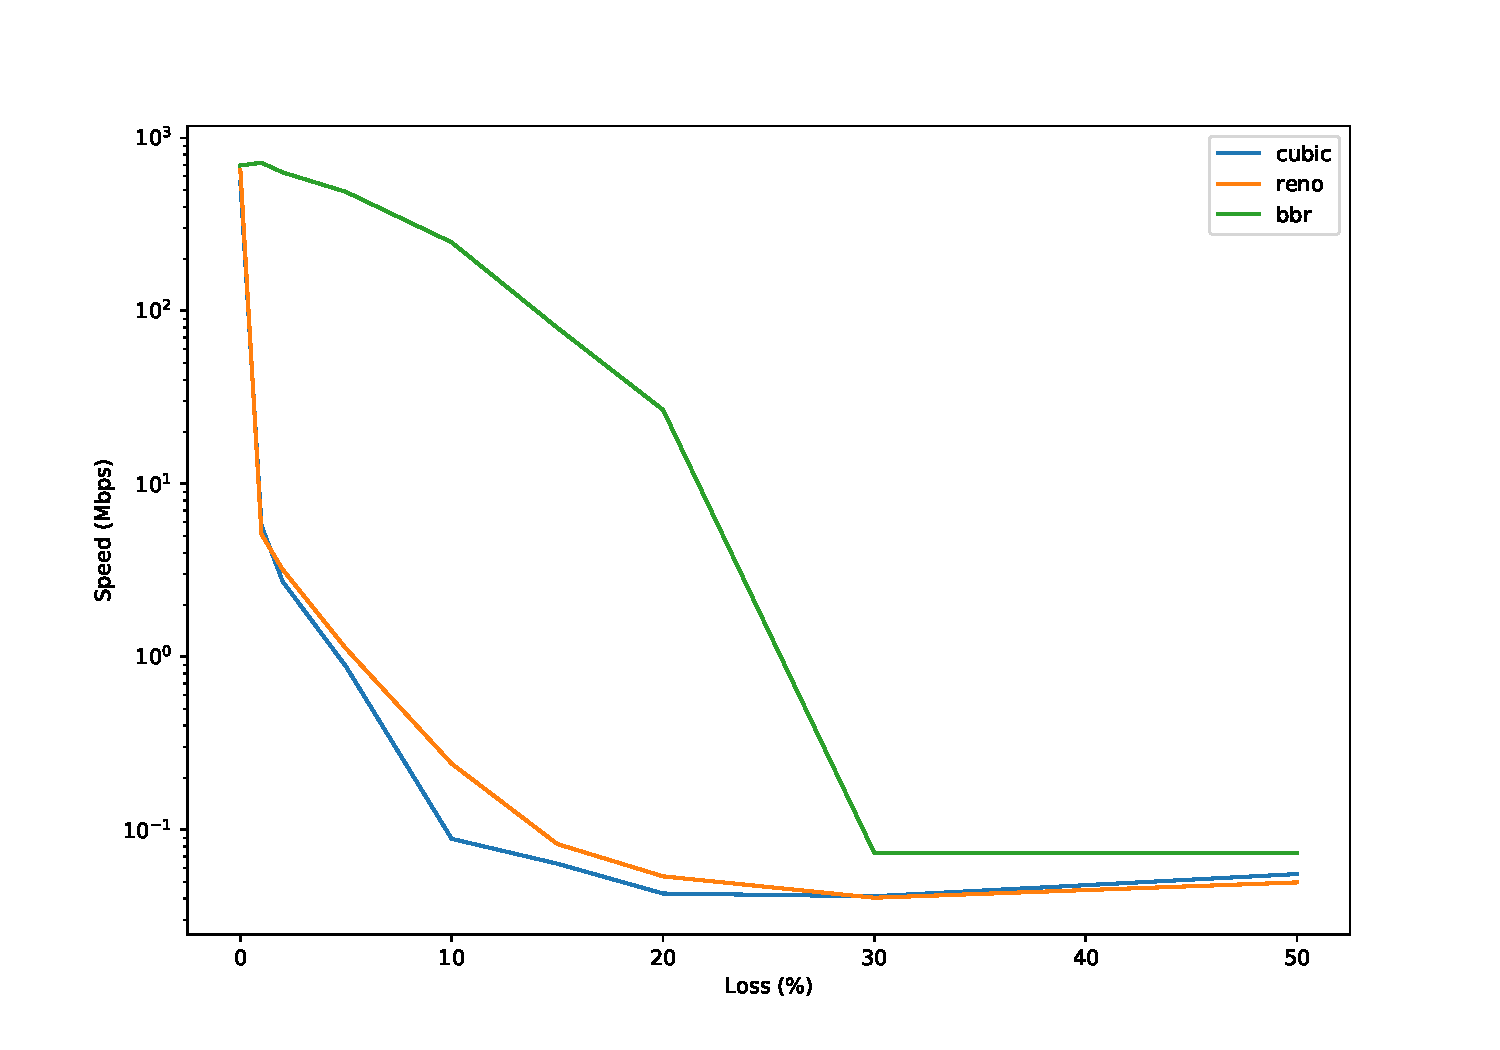
\includegraphics[width=\textwidth,height=\textheight,keepaspectratio]{../iperf_test/plot_log.pdf}
  \end{figure}
\end{frame}

\begin{frame}{20 seconds Iperf test: speed vs loss distribution [3/5]}
  \begin{figure}
	  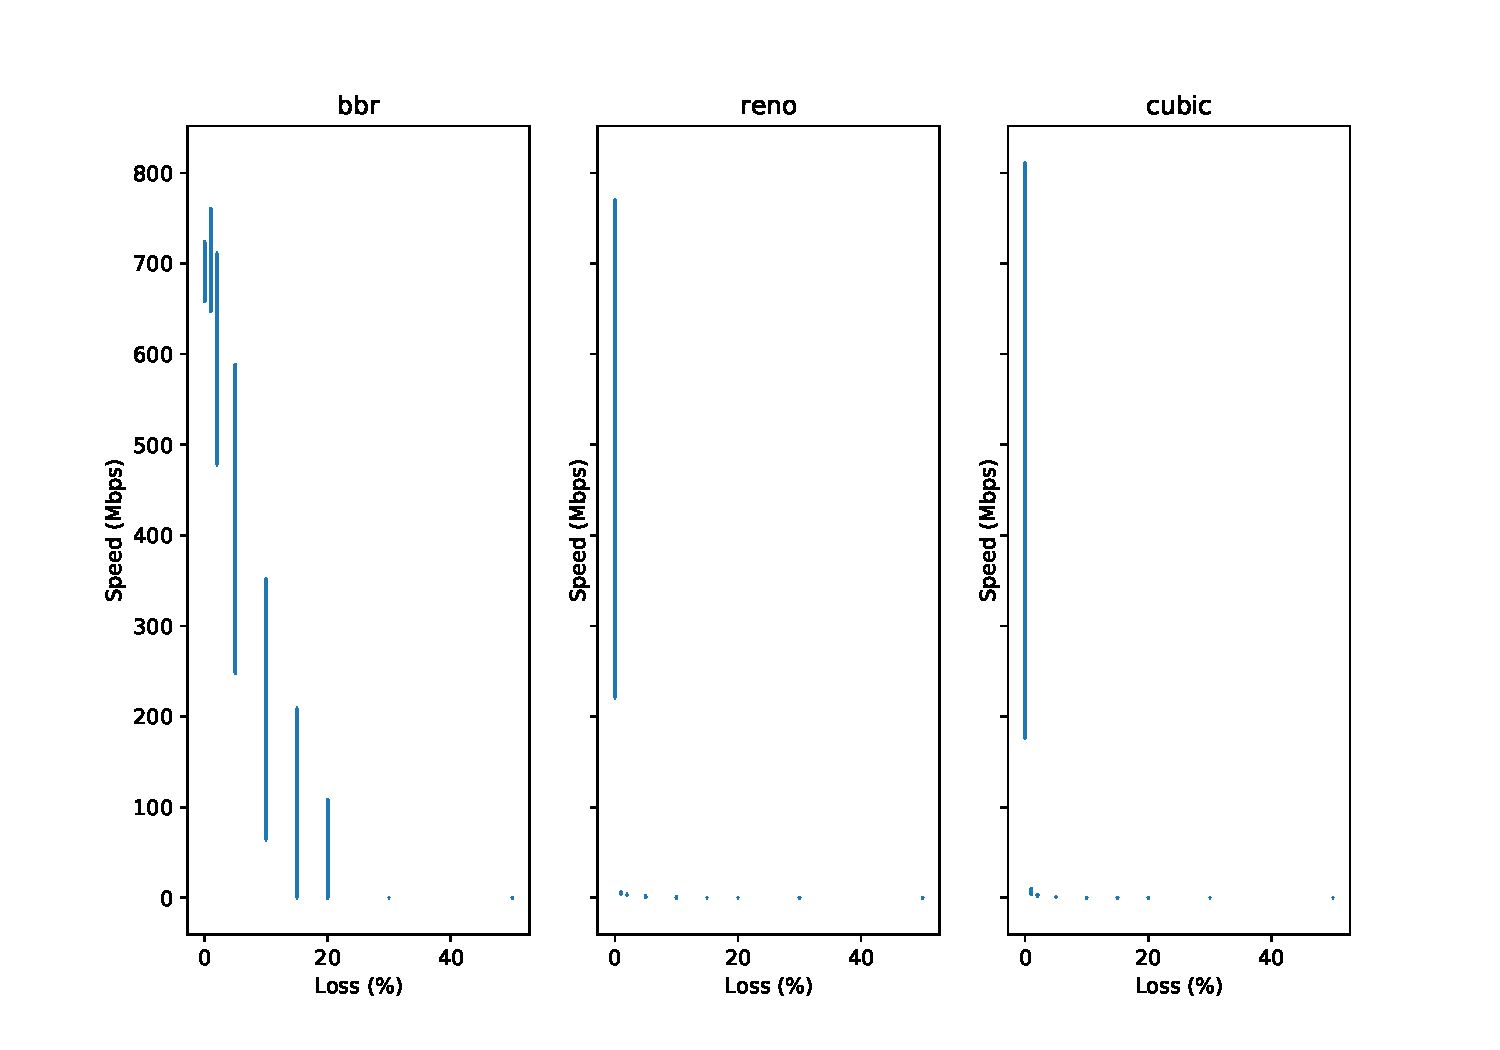
\includegraphics[width=\textwidth,height=\textheight,keepaspectratio]{../iperf_test/violinplot.pdf}
  \end{figure}
\end{frame}


\begin{frame}{20 seconds Iperf test: speed vs delay (log) [4/5]}
  \begin{figure}
	  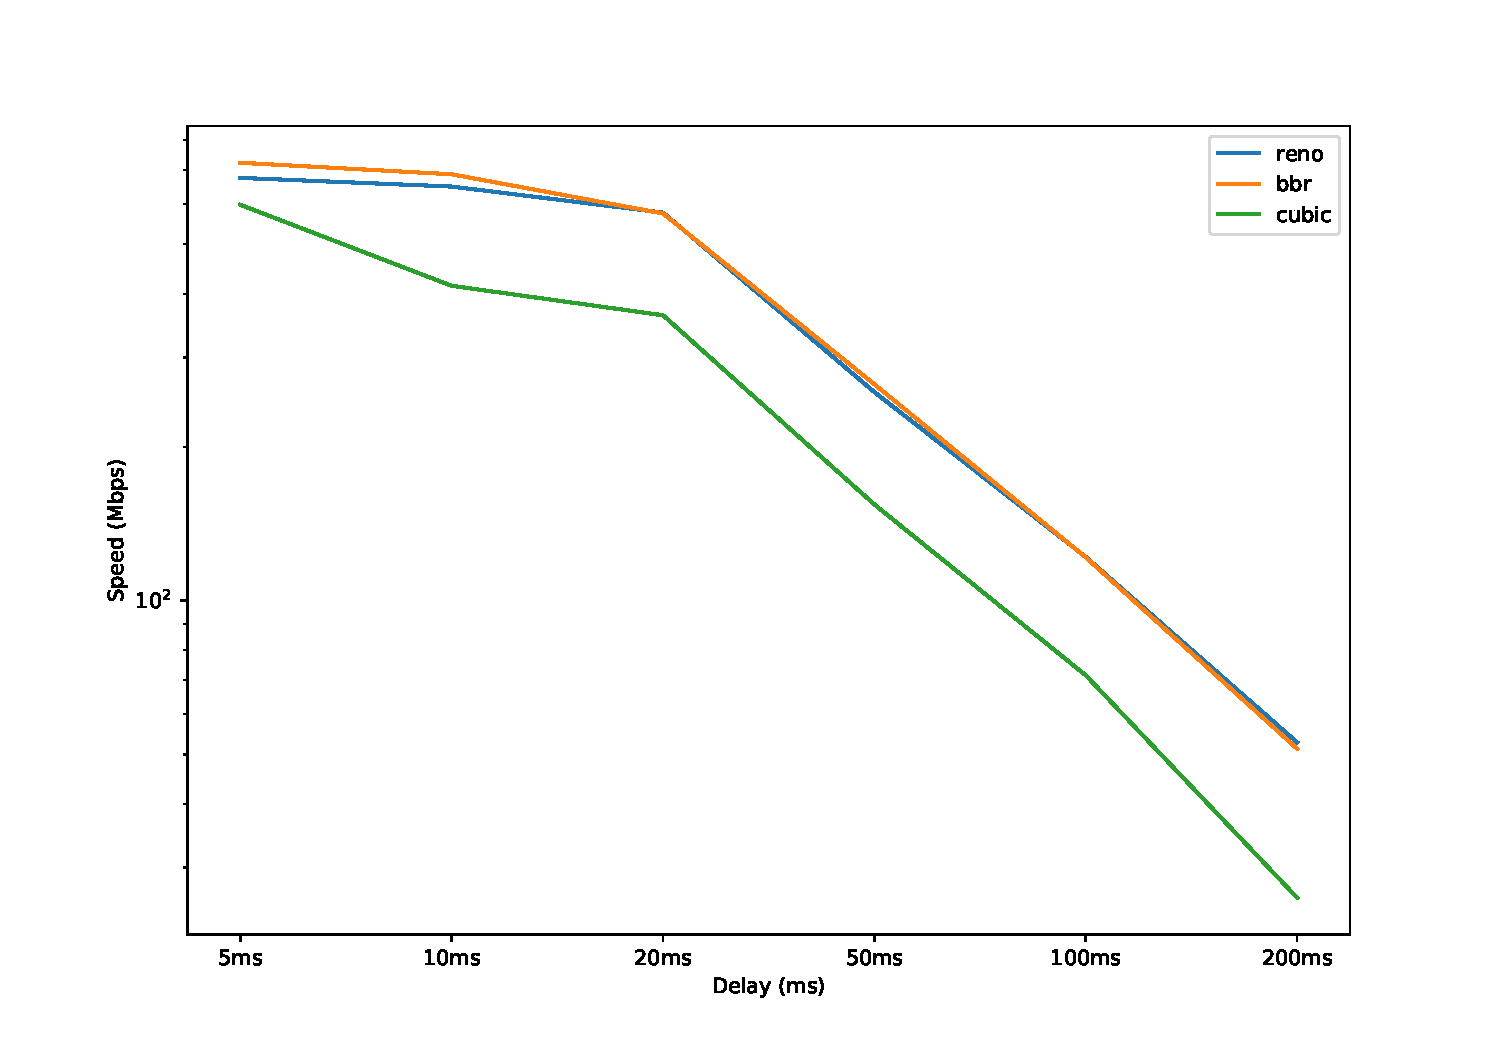
\includegraphics[width=\textwidth,height=\textheight,keepaspectratio]{../iperf_test_delay/plot_log.pdf}
  \end{figure}
\end{frame}

\begin{frame}{20 seconds Iperf test: speed vs delay distribution [5/5]}
  \begin{figure}
	  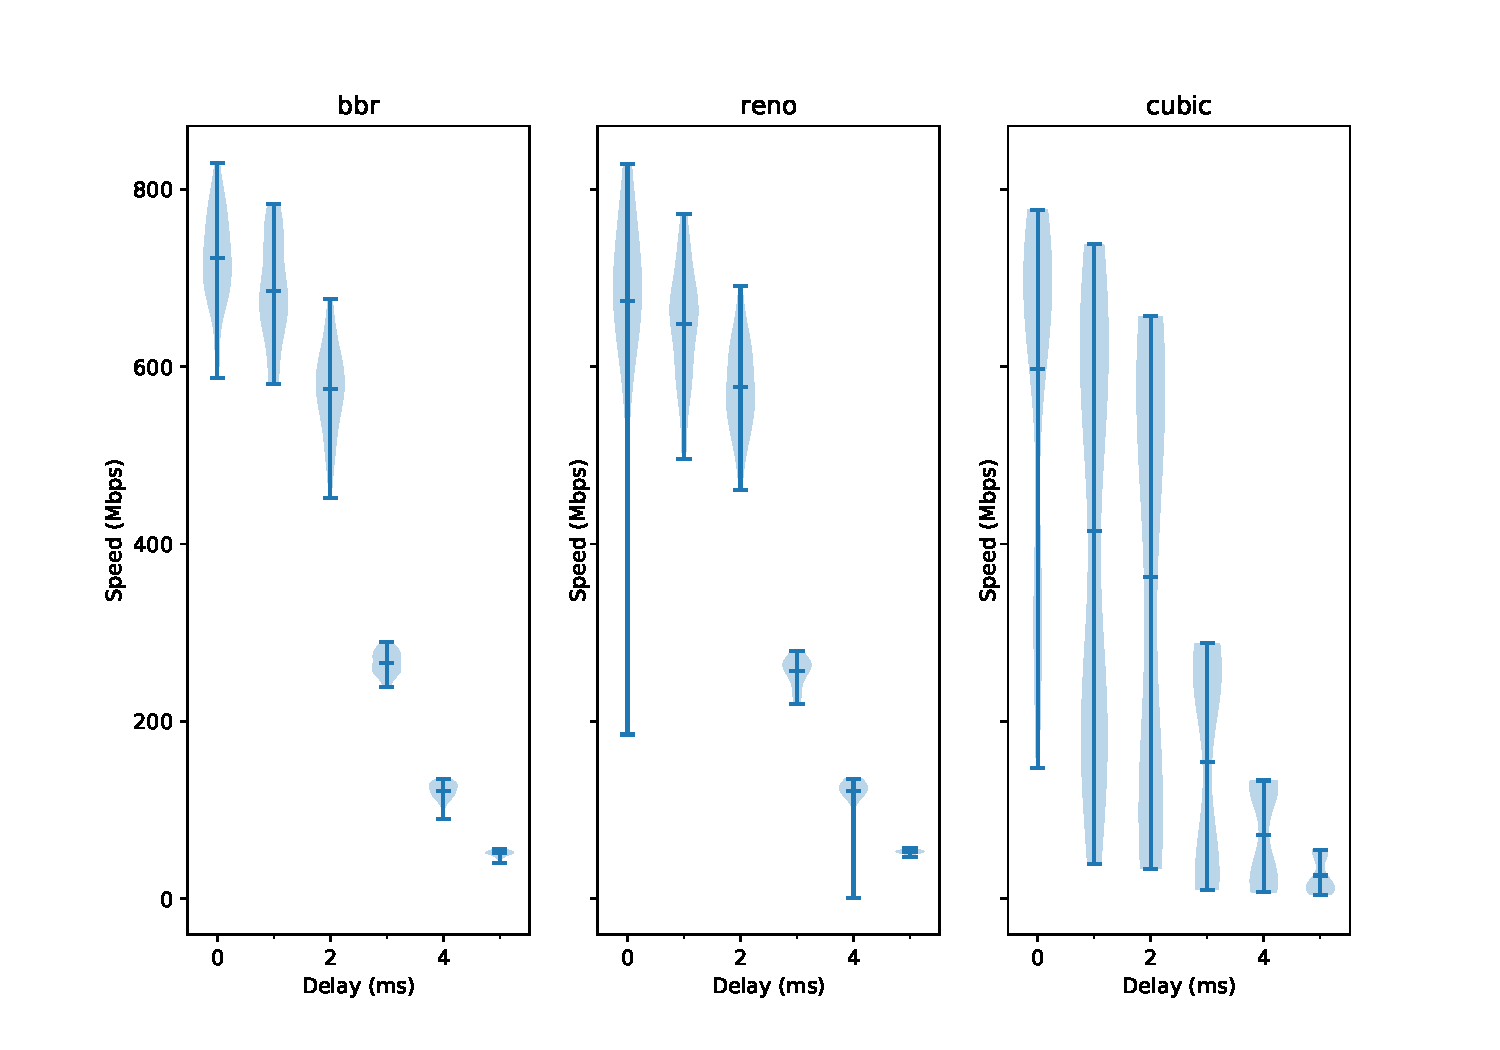
\includegraphics[width=\textwidth,height=\textheight,keepaspectratio]{../iperf_test_delay/violinplot.pdf}
  \end{figure}
\end{frame}


\begin{frame}{Complex web page simulation: description [1/4]}
	\begin{itemize}

		\item Variable loss rate on the server's link
		\item \texttt{h1} as server
		\item \texttt{h2} as client
		\item \texttt{nginx} as server since Python's \texttt{SimpleHTTPServer} is too slow
		\item \texttt{wget -r} as client, simulating the web page browsing
		\item \texttt{bbc.co.uk} index page as an example: elements has same size but random data
		\item 72 elements with a total size of 2.902 MB
		\item Speed is obviously slower than a single big file download
		\item Elements included as images into a simple HTML file
	\end{itemize}
\end{frame}

\begin{frame}{Complex web page simulation: page structure [2/4]}
  \begin{figure}
	  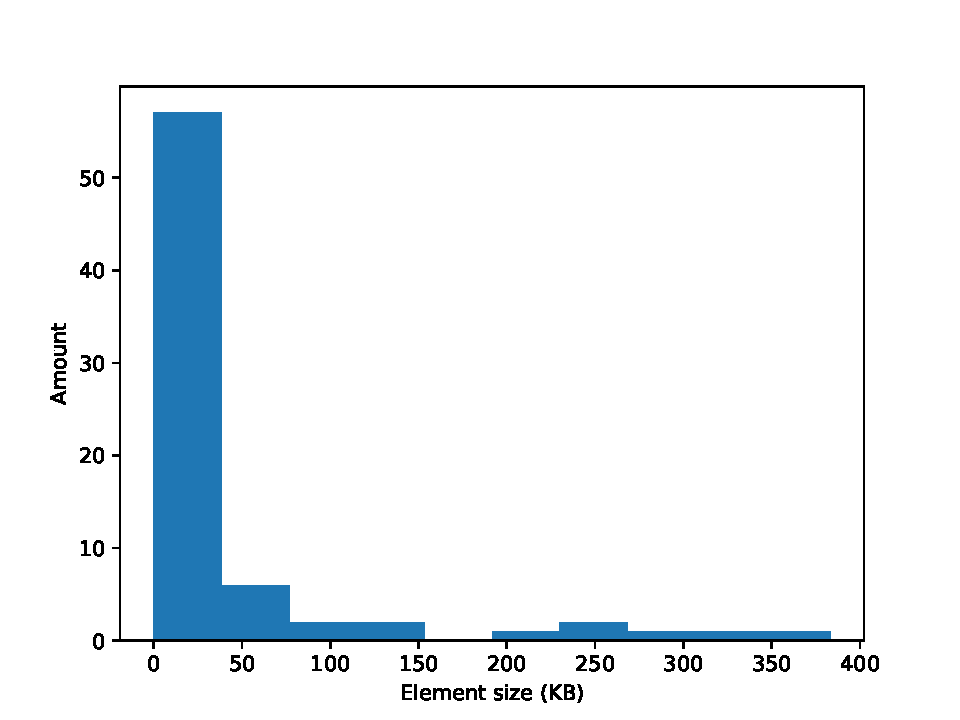
\includegraphics[width=\textwidth,height=\textheight,keepaspectratio]{../http_test/page_stat.pdf}
  \end{figure}

\end{frame}



\begin{frame}{Complex web page simulation: speed (log) [4/4]}
  \begin{figure}
	  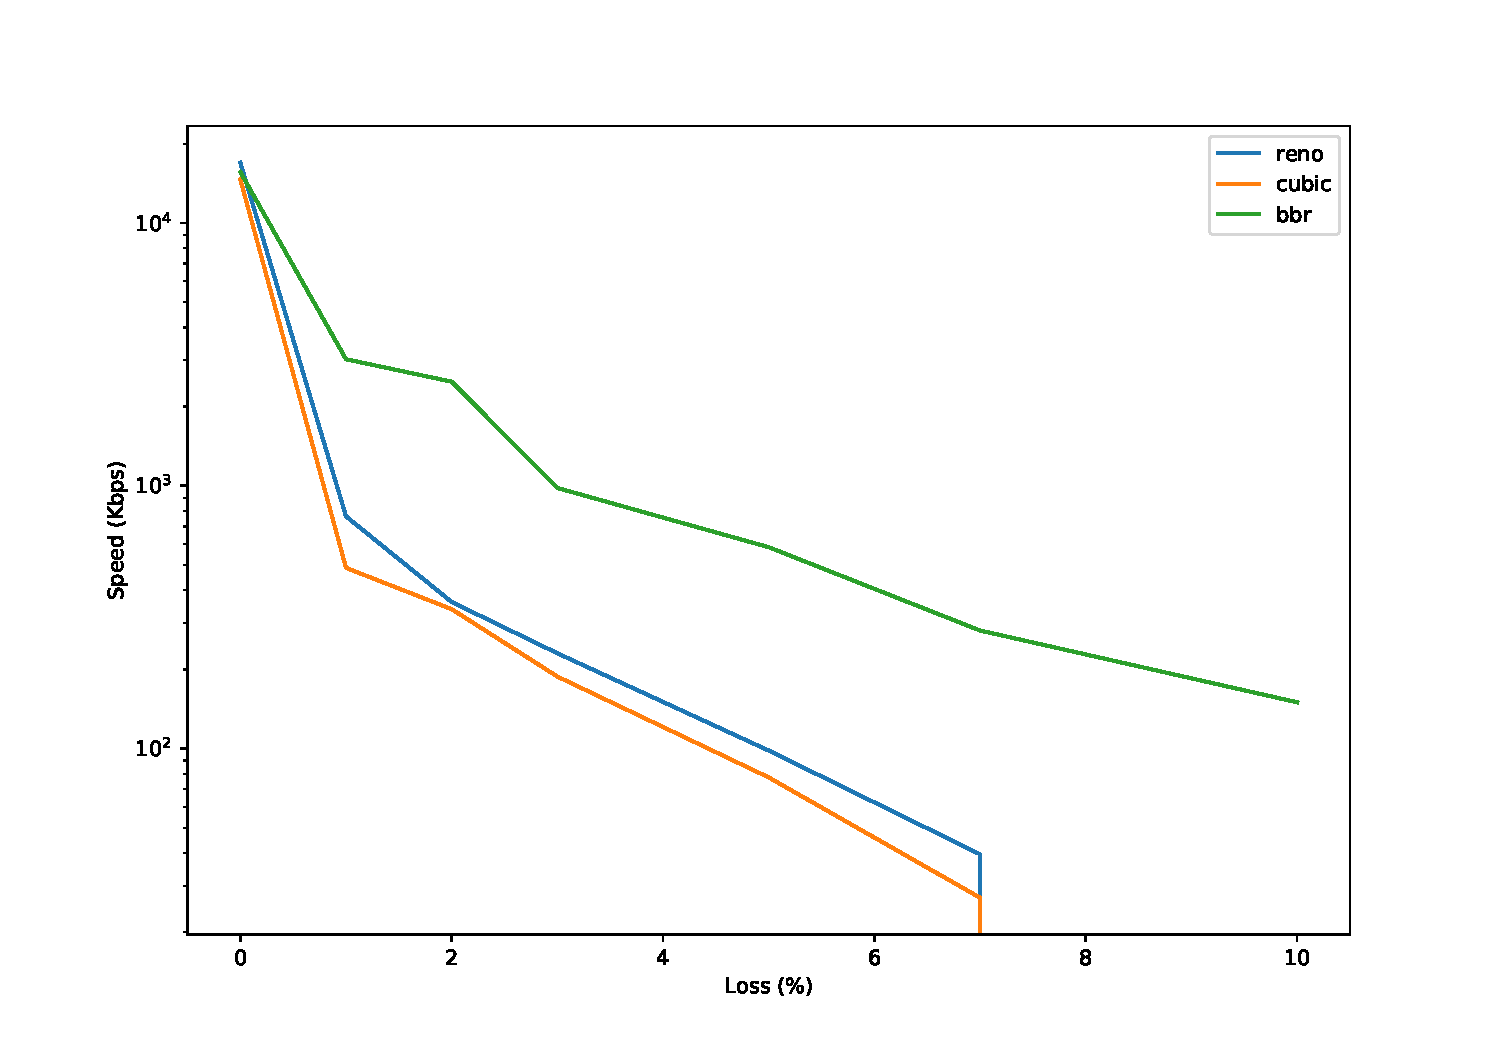
\includegraphics[width=\textwidth,height=\textheight,keepaspectratio]{../http_test/plot_log.pdf}
  \end{figure}
\end{frame}

\begin{frame}{Complex web page simulation: speed distribution [4/4]}
  \begin{figure}
	  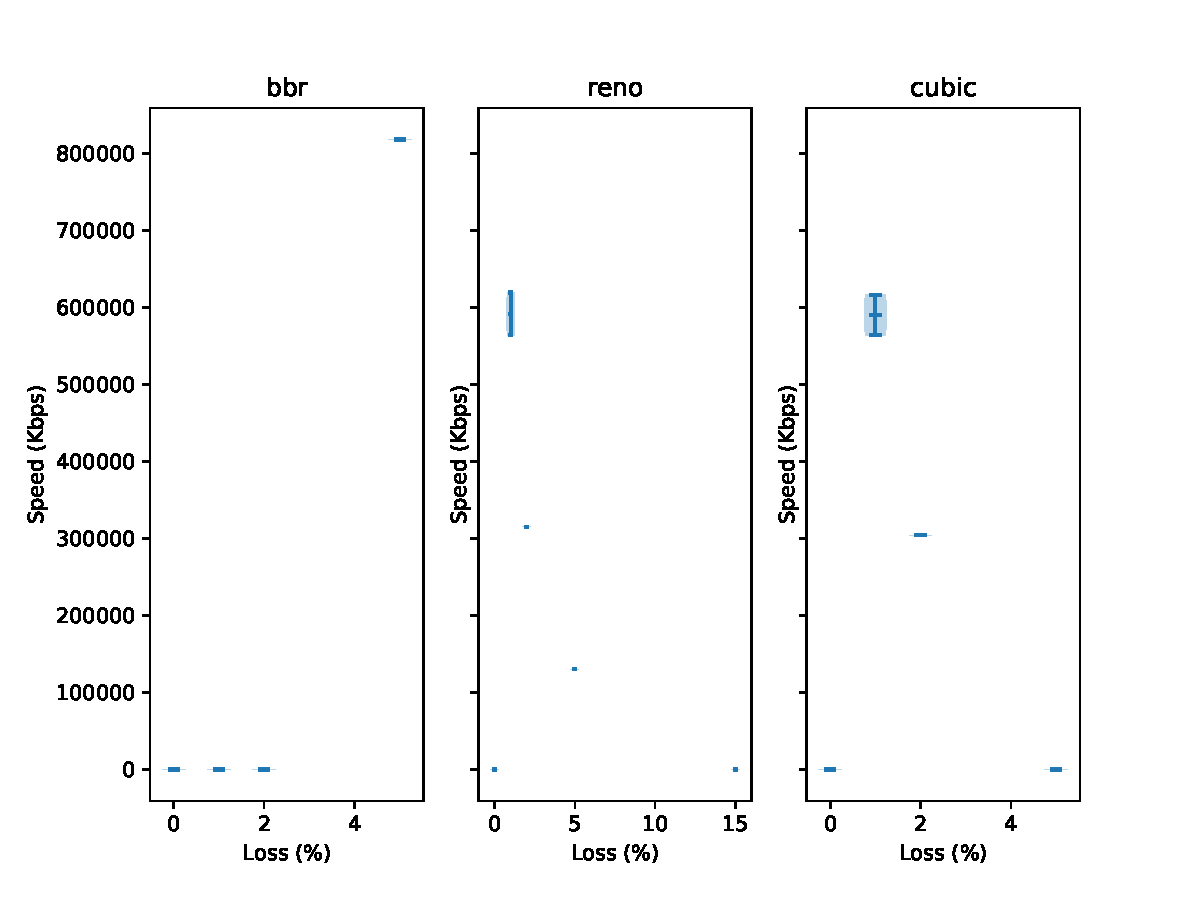
\includegraphics[width=\textwidth,height=\textheight,keepaspectratio]{../http_test/violinplot.pdf}
  \end{figure}
\end{frame}




\begin{frame}{Single file download: description}
		\begin{itemize}
			\item Variable loss rate on the server's link
			\item \texttt{h1} as server
			\item \texttt{h2} as client
			\item As before, \texttt{nginx} as server
			\item Simple \texttt{wget} as client, 120 seconds timeout
			\item 500KB, 1MB, 2MB, 5MB, 10MB and 100MB files
			\item Random content in files
		\end{itemize}
\end{frame}

\begin{frame}{Single file download: speed for every size and protocol [1/2]}
  \begin{figure}
	  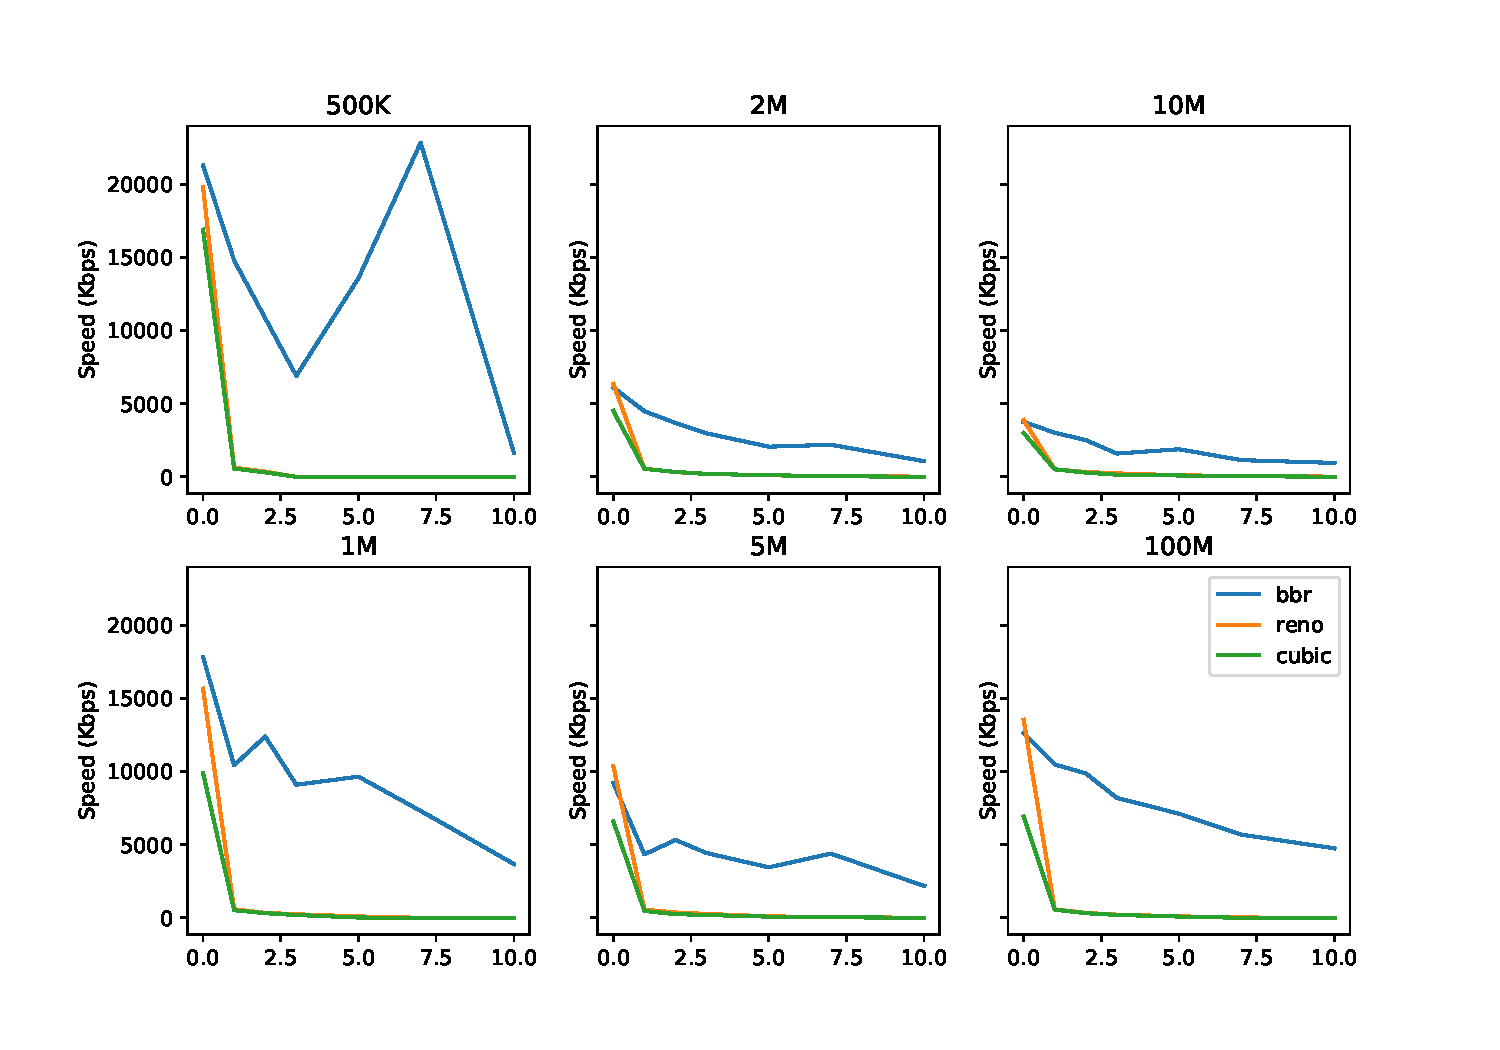
\includegraphics[width=\textwidth,height=\textheight,keepaspectratio]{../http_single_test/sizes_plot.pdf}
  \end{figure}
\end{frame}

\begin{frame}{Single file download: BBR performances [2/2]}
  \begin{figure}
	  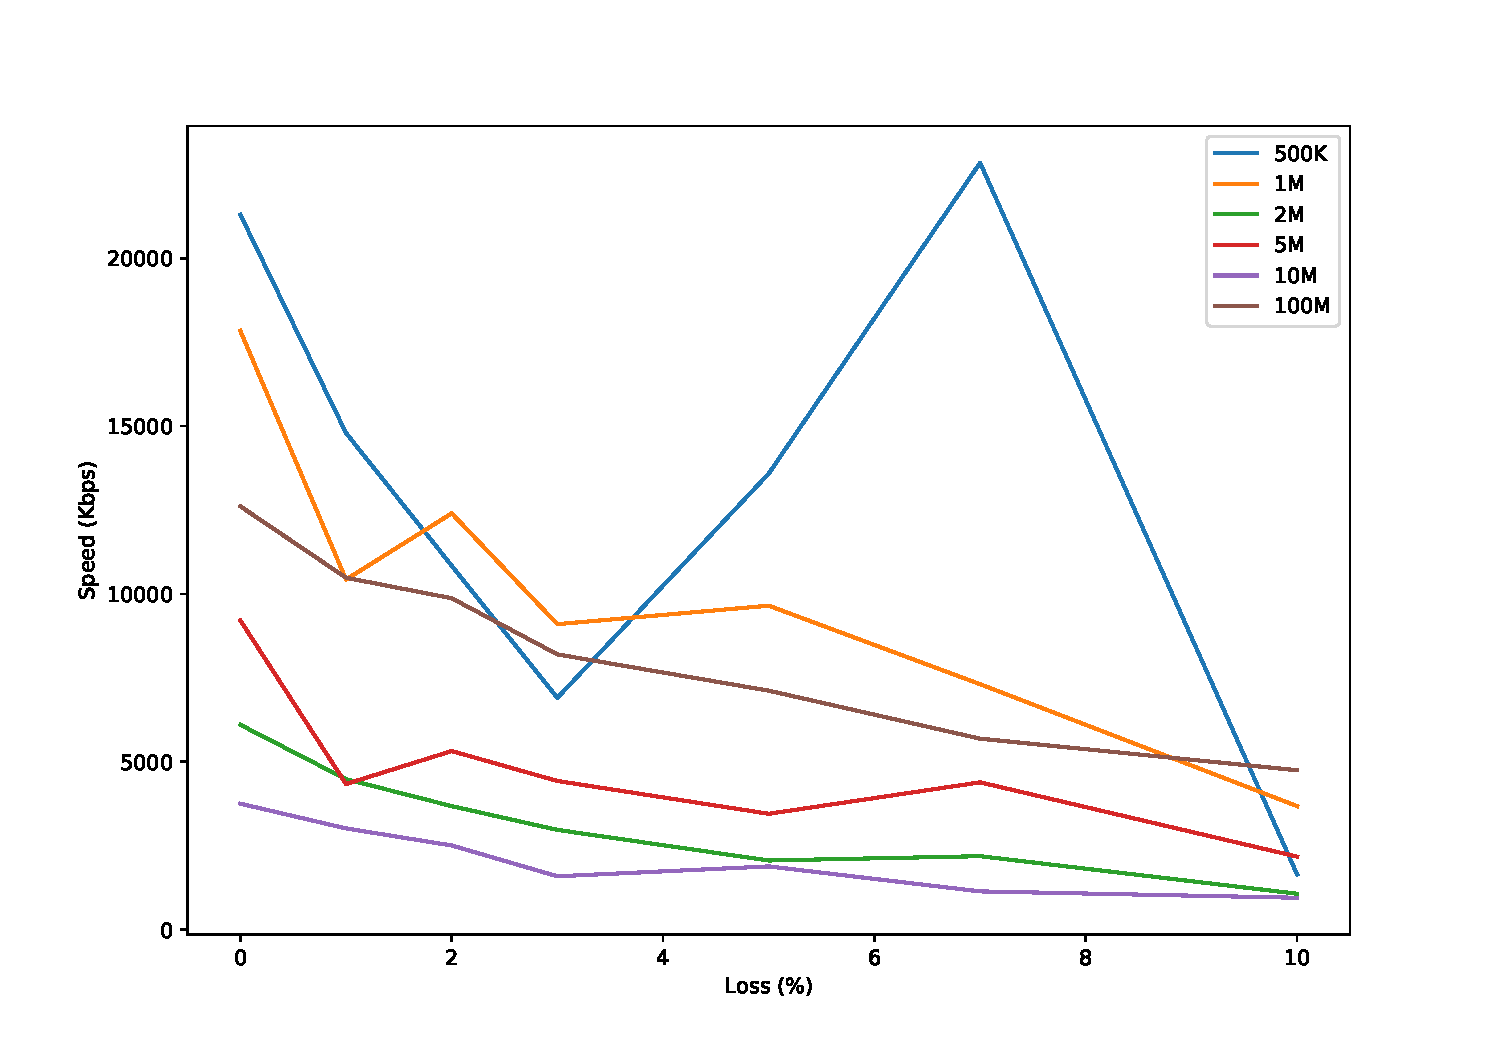
\includegraphics[width=\textwidth,height=\textheight,keepaspectratio]{../http_single_test/size_bbr_plot.pdf}
  \end{figure}
\end{frame}


\begin{frame}{New Reno faster than Cubic!? [1/2]}
	From the previous tests, it appears that New Reno is faster than Cubic in some cases.
	I run some test on a real network, just to verify.
	\begin{itemize}
		\item 1 Gbit links, adequate hardware
		\item less than 1 ms ping time
		\item Debian with 4.18 kernel on same machines
		\item Overall, New Reno appeared up to 5 Mbps faster than Cubic
		\item Limited tests and environment variables: longer tests should be performed
		\item Of course, it can depend by specific version or machine's characteristics
	\end{itemize}
\end{frame}

\begin{frame}{New Reno faster than Cubic!? [2/2]}
\begin{table}[]
\begin{tabular}{l|l|l}
\textbf{Condition} & \textbf{New Reno} & \textbf{Cubic} \\ \hline
No delay, no loss  & 947               & 942            \\
100 ms delay       & 201               & 196            \\
5\% loss           & 944               & 942            \\
10\% loss          & 943               & 913           
\end{tabular}
\end{table}
\end{frame}

\begin{frame}{Conclusions}
	\begin{itemize}
		\item Tests showed the better performances of BBR over Cubic and New Reno
		\item BBR achieves better speed both across loss and delays
		\item Congestion Window cannot be inspected without rebuilding the kernel (to get \texttt{tcp\_probe})
		\item Fairness to other protocols needs to be investigated using multiple machines (the kernel is shared)
        \item All the code is available on \url{github.com/MassimoGirondi/DNCS_BBR}.
	\end{itemize}
\end{frame}



\end{document}
